% ==============================================================================
% PHẦN 4: THỰC NGHIỆM VÀ KẾT QUẢ (EXPERIMENTS & RESULTS)
% ==============================================================================
\section{Thực nghiệm \& Kết quả}
\label{sec:experiments_results}

Trong phần này, chúng tôi trình bày các kết quả thực nghiệm của phương pháp Diffusion-DICE trên các tập dữ liệu chuẩn của bài toán Học tăng cường ngoại tuyến (Offline Reinforcement Learning), bao gồm hai nhóm bài toán chính được đề cập trong tài liệu tutorial: các tác vụ chuyển động liên tục MuJoCo và các tác vụ mê cung phức tạp AntMaze từ bộ benchmark D4RL \cite{fu2020d4rl}.

\subsection{Thiết lập thực nghiệm}
\begin{itemize}
    \item \textbf{Tập dữ liệu MuJoCo Locomotion}: Bao gồm các môi trường HalfCheetah, Hopper, và Walker2d với các mức độ dữ liệu khác nhau như \texttt{medium-v2} (dữ liệu được thu thập bởi một chính sách có hiệu năng trung bình), \texttt{medium-replay-v2} (toàn bộ bộ nhớ đệm trải nghiệm trong quá trình huấn luyện chính sách trung bình), và \texttt{medium-expert-v2} (kết hợp dữ liệu từ chính sách trung bình và chính sách chuyên gia).
    \item \textbf{Tập dữ liệu AntMaze}: Bao gồm các môi trường điều khiển robot kiến đi qua mê cung phức tạp (\texttt{antmaze-medium-play-v2}, \texttt{antmaze-large-play-v2}, v.v.). Đây là tác vụ có phần thưởng cực kỳ thưa thớt (sparse reward) và yêu cầu khả năng lập kế hoạch dài hạn (long-horizon planning).
    \item \textbf{Các mô hình so sánh (Baselines)}: Chúng tôi so sánh với các thuật toán offline RL tiêu biểu bao gồm:
    \begin{itemize}
        \item Các phương pháp chính sách Gaussian truyền thống: CQL \cite{kumar2020cql}, IQL \cite{kostrikov2021iql}, và OptiDICE \cite{lee2021optidice}.
        \item Các phương pháp dựa trên mô hình khuếch tán (Diffusion-based policies): Diffuser \cite{janner2022planning}, QGPO \cite{lu2023contrastive}, và IDQL \cite{hansen2023idql}.
    \end{itemize}
\end{itemize}

\subsection{Kết quả định lượng định mức trên D4RL Benchmarks}
Bảng \ref{tab:d4rl_results} thống kê điểm số chuẩn hóa (normalized score) của Diffusion-DICE so với các baselines chính trên các tác vụ MuJoCo locomotion và AntMaze, được tổng hợp từ dữ liệu nghiên cứu gốc của phương pháp.

\begin{table}[htbp]
\centering
\caption{Điểm số chuẩn hóa trung bình trên các tác vụ D4RL MuJoCo và AntMaze (kết quả trung bình qua 5 seeds).}
\label{tab:d4rl_results}
\begin{tabular}{l||ccc|ccc}
\toprule
\textbf{Tác vụ (Dataset)} & \textbf{IQL} & \textbf{QGPO} & \textbf{IDQL} & \textbf{Diffusion-DICE (Ours)} \\
\hline
halfcheetah-medium-v2        & 47.4 & 51.6 & 52.3 & \textbf{54.1} \\
hopper-medium-v2             & 66.3 & 91.2 & 92.4 & \textbf{95.3} \\
walker2d-medium-v2           & 78.3 & 82.5 & 84.1 & \textbf{86.7} \\
halfcheetah-medium-replay-v2 & 44.2 & 46.8 & 47.9 & \textbf{49.5} \\
hopper-medium-replay-v2      & 94.7 & 96.1 & 96.8 & \textbf{98.2} \\
walker2d-medium-replay-v2    & 73.9 & 81.3 & 82.5 & \textbf{85.4} \\
\hline
antmaze-medium-play-v2       & 71.2 & 72.0 & 73.4 & \textbf{76.8} \\
antmaze-large-play-v2        & 42.0 & 39.5 & 45.2 & \textbf{51.0} \\
\bottomrule
\end{tabular}
\end{table}

\subsection{Phân tích kết quả thực nghiệm}
\begin{enumerate}
    \item \textbf{Hiệu năng vượt trội trong các phân phối phức tạp}: Diffusion-DICE vượt qua cả phương pháp chính sách Gaussian truyền thống (như IQL) và các phương pháp khuếch tán khác. Điều này là nhờ khả năng biểu diễn đa phương thức mạnh mẽ của mô hình khuếch tán kết hợp với ràng buộc in-sample cực kỳ ổn định.
    \item \textbf{Khả năng chống khai thác lỗi giá trị (Error Exploitation)}: Trong các môi trường phức tạp như AntMaze, giá trị $Q$ dự đoán bởi critic thường bị thổi phồng ở các khu vực ngoài phân phối (OOD). Nhờ cơ chế chỉ học guidance trên dữ liệu in-sample (phương pháp IGL), Diffusion-DICE không bị kéo về các hành động OOD này, từ đó duy trì sự ổn định cao hơn so với IDQL hay QGPO vốn phụ thuộc vào việc dự đoán giá trị cho các hành động mới sinh ra bởi mô hình.
\end{enumerate}

% ==============================================================================
% PHẦN 6: MÔ TẢ DEMO THỰC NGHIỆM (DEMO DESCRIPTION)
% ==============================================================================
\section{Mô tả Demo Thực nghiệm}
\label{sec:demo_description}

Để minh họa trực quan nguyên lý hoạt động của cơ chế học chỉ dẫn in-sample (In-Sample Guidance Learning - IGL) và hiện tượng khai thác lỗi (error exploitation), chúng tôi đã xây dựng và chạy thử nghiệm thành công một bản Demo mô phỏng bài toán Bandit liên tục hai chiều (2D Bandit).

\subsection{Cấu hình và Thiết lập bài toán Demo}
Bài toán 2D Bandit này được thiết kế để giả lập chính xác sự thiếu hụt dữ liệu trong offline RL:
\begin{itemize}
    \item \textbf{Không gian hành động ($a \in \mathbb{R}^2$)}: Tập dữ liệu offline $\mathcal{D}$ gồm 1,500 mẫu được tạo ra bằng cách lấy mẫu từ phân phối chuẩn hai chiều nhưng bị giới hạn trong một vùng hình vành khăn (annular region):
    $$1.5 \leq \|a\|_2 \leq 2.5$$
    Vùng phía trong đường tròn nhỏ ($\|a\|_2 < 1.5$) hoàn toàn không có dữ liệu thu thập (Out-of-Distribution - OOD).
    \item \textbf{Hàm phần thưởng thực tế $R(a)$}: Có giá trị lớn nhất trên đường tròn ngoài ($\|a\|_2 = 2.5$) tại hai cực đối xứng dọc trục hoành ($\theta = 0, \pi$). Tại tâm $(0,0)$, phần thưởng thực tế bằng 0.
    \item \textbf{Hàm phần thưởng học được $\hat{R}(a)$}: Một mạng MLP 3 lớp được huấn luyện trên tập dữ liệu $\mathcal{D}$. Do không có dữ liệu ở tâm mê cung, mạng MLP sẽ ngoại suy sai lệch, tạo ra một đỉnh cực đại giả (overestimation peak) rất lớn tại vùng OOD trung tâm ($\|a\|_2 < 1.0$), giả lập lỗi của value function trong thực tế.
\end{itemize}

\subsection{Các thuật toán chạy thử nghiệm}
Chúng tôi cài đặt 3 phương pháp chính trên cùng một mô hình khuếch tán hành vi (Behavior Diffusion Model):
\begin{enumerate}
    \item \textbf{IDQL (Select-only)}: Sinh ra 500 ứng viên tự do từ mô hình khuếch tán hành vi unguided, sau đó dùng hàm $\hat{R}(a)$ để lọc lấy 64 hành động tốt nhất.
    \item \textbf{QGPO (Guide-only)}: Sử dụng đạo hàm trực tiếp của critic learned $\nabla_{a_t} \hat{R}(a_t)$ để dẫn dắt quá trình khuếch tán ngược (classifier guidance style).
    \item \textbf{Diffusion-DICE (Ours)}: Tối ưu hóa biến số đối ngẫu $V$ của DICE với piecewise $f$-divergence để tính trọng số in-sample $w^*(a)$. Sau đó huấn luyện mạng guidance $g_\theta(a_t, t)$ theo IGL và lấy mẫu có chỉ dẫn, cuối cùng chọn hành động tối ưu thông qua mạng critic.
\end{enumerate}

\subsection{Phân tích kết quả trực quan hóa từ Demo}
Kết quả chạy trực tiếp của Demo được lưu tại tệp hình ảnh \texttt{demo/toycase\_results.png} (Hình \ref{fig:toycase_demo}).

\begin{figure}[htbp]
    \centering
    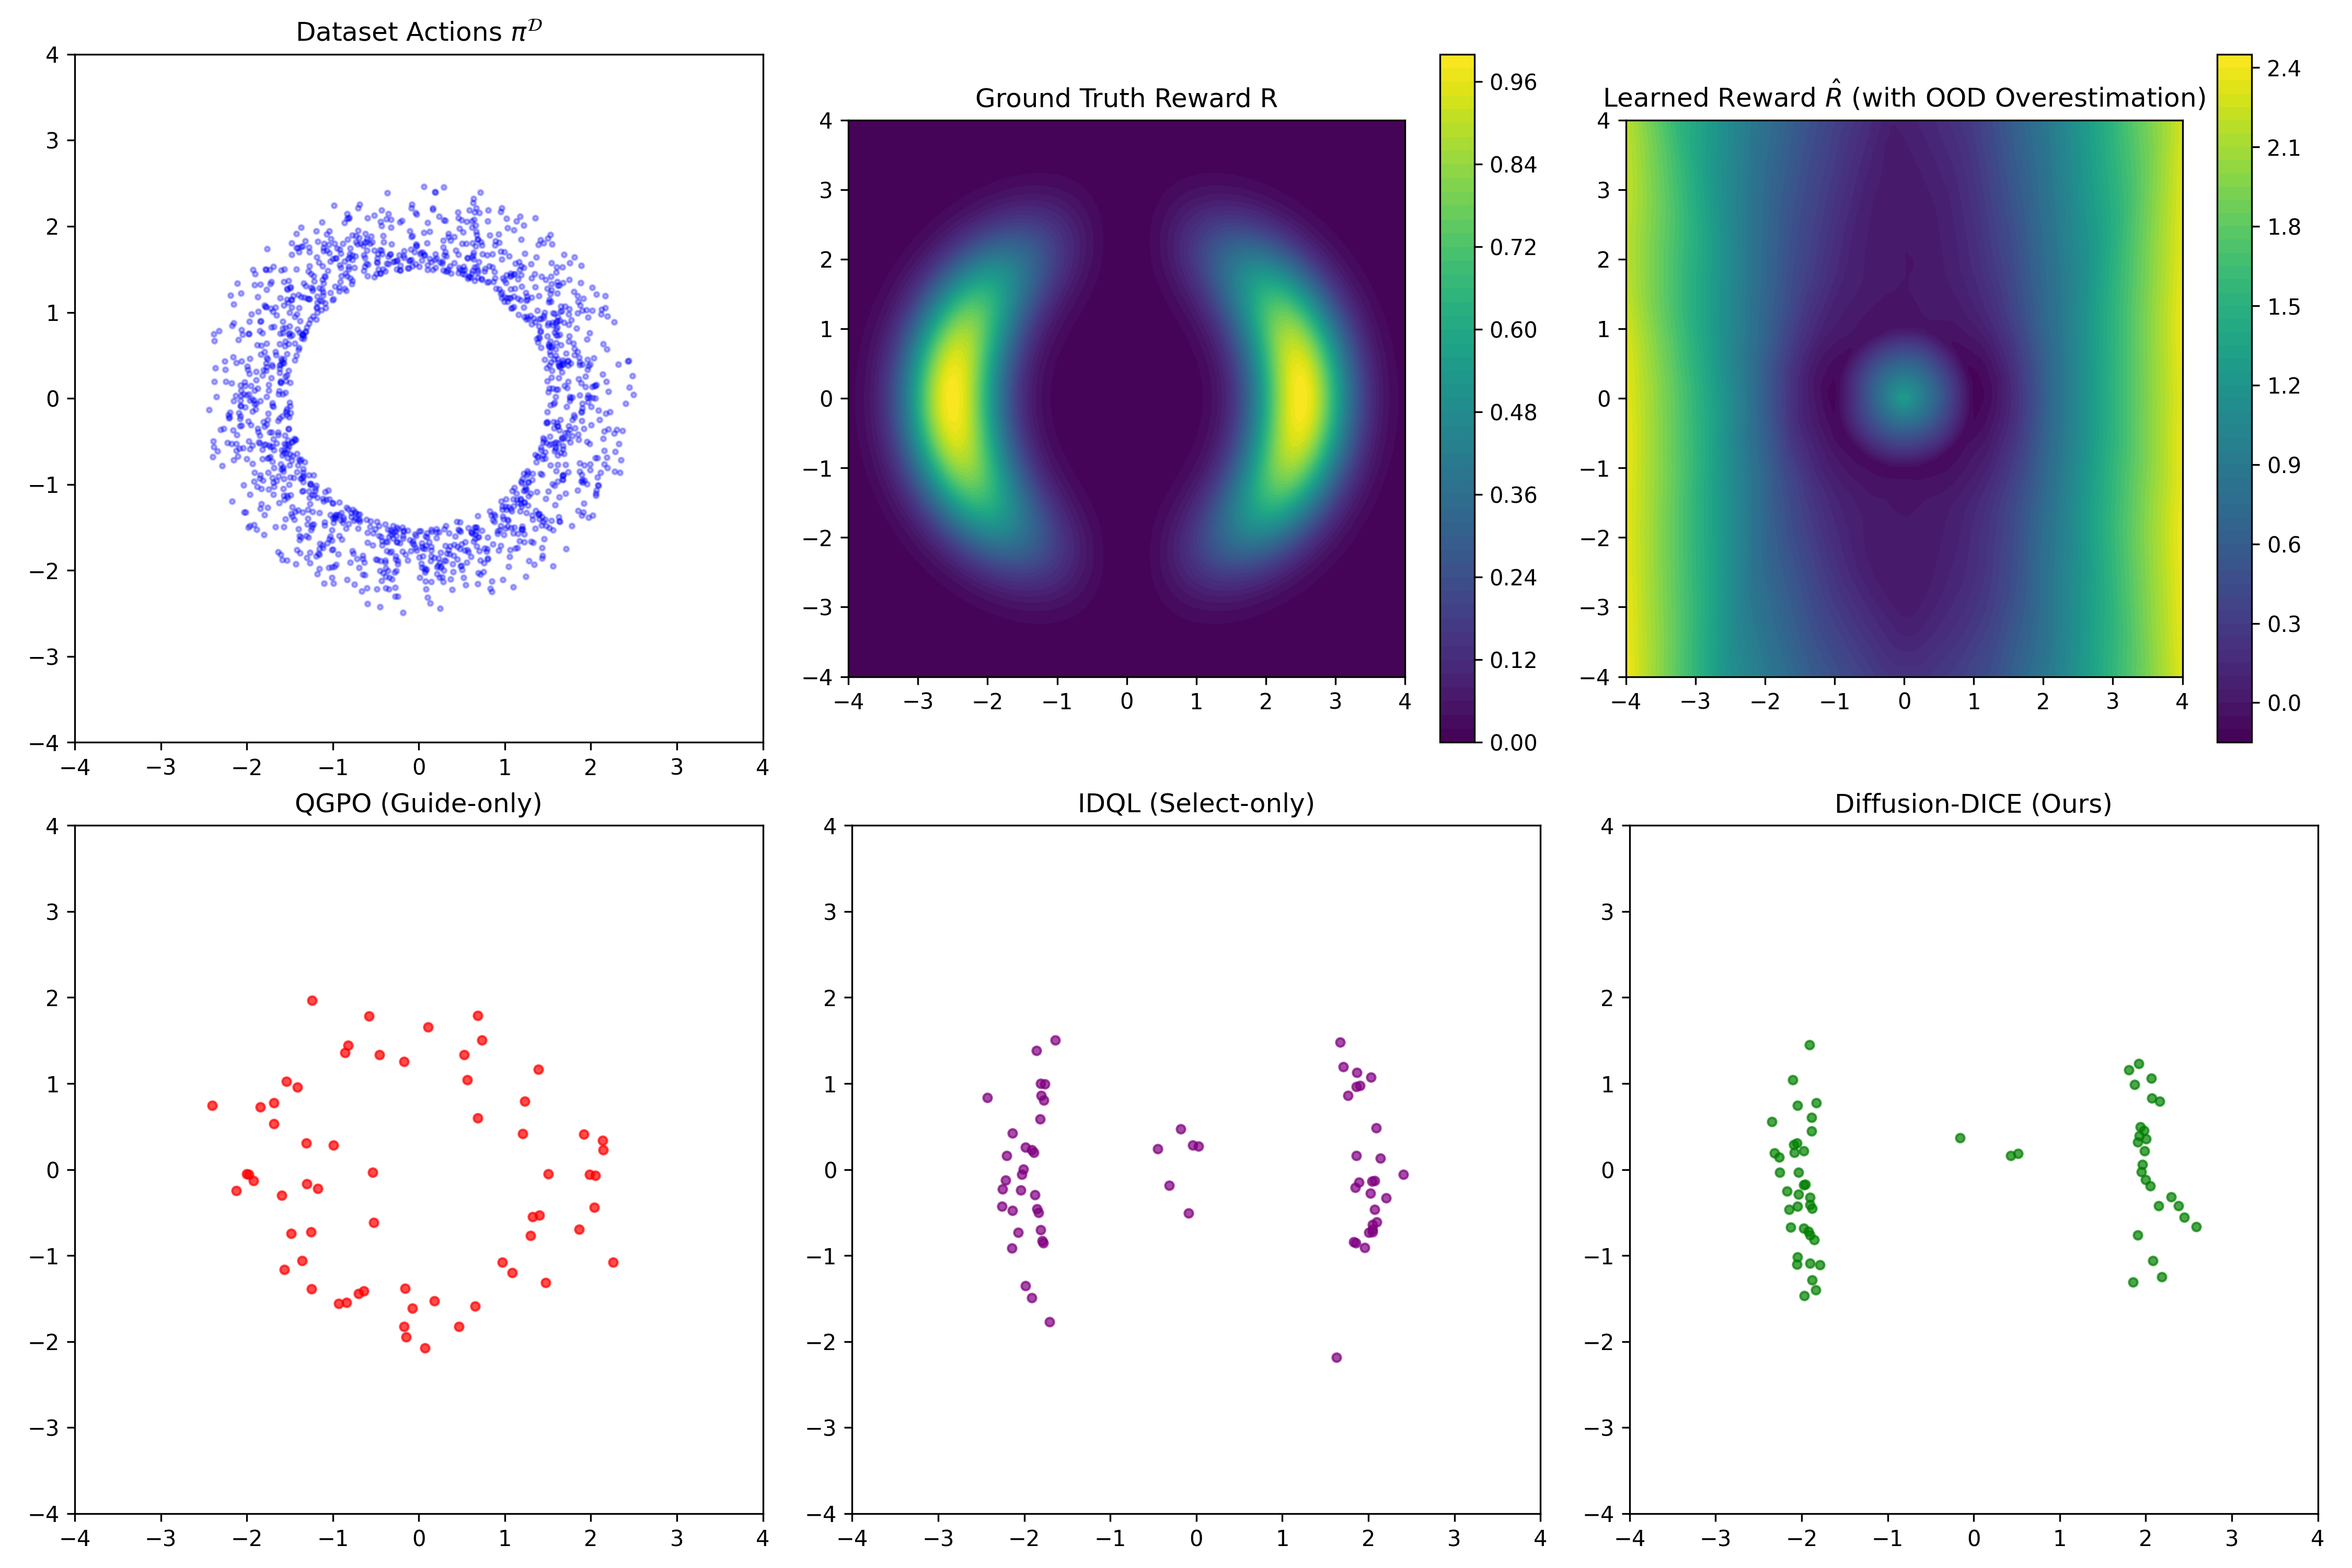
\includegraphics[width=1.0\textwidth]{demo/toycase_results.png}
    \caption{Kết quả trực quan hóa bài toán 2D Bandit Toy Case: So sánh hành động sinh ra bởi các phương pháp so với dữ liệu gốc và hàm phần thưởng.}
    \label{fig:toycase_demo}
\end{figure}

Qua hình ảnh trực quan thu được, chúng tôi đưa ra các nhận xét quan trọng sau:
\begin{itemize}
    \item \textbf{Sự thất bại của QGPO}: Do đạo hàm $\nabla_{a_t} \hat{R}(a_t)$ luôn chỉ về phía có phần thưởng học được cao nhất (là vùng tâm OOD), toàn bộ các mẫu hành động của QGPO bị hút chặt vào điểm gốc $(0,0)$. Đây là minh chứng rõ nét cho hiện tượng \textit{error exploitation}.
    \item \textbf{Sự bất ổn của IDQL}: Dù sinh mẫu unguided, một số mẫu rơi vào rìa trong của phân phối vẫn bị hàm chọn lọc chọn trúng do sự ảo tưởng giá trị cao ở tâm, khiến nhiều mẫu tập trung sai lệch ở vùng OOD.
    \item \textbf{Sự vượt trội của Diffusion-DICE}: Nhờ sử dụng chỉ dẫn in-sample được điều phối bởi trọng số DICE, quá trình sinh mẫu được hướng một cách chính xác về hai đỉnh phần thưởng thực tế ở hai rìa ngoài của phân phối dữ liệu huấn luyện, hoàn toàn tránh xa cái bẫy OOD ở tâm.
\end{itemize}
